Giovanni \citeonline{mori_analysing_2015} perspetivou a importância da Música para os \emph{live coders} de um ponto-de-vista etnongráfico, ao apontar locais e costumes onde o \emph{live coding} é praticado:

\begin{citacao}
\emph{Live coding} é uma técnica artística de improvisação. Pode ser empregada em muitos contextos performativos diferentes: dança, música, imagens em movimento e mesmo tecelagem. Concentrei minha atenção no lado musical, que parece ser o mais proeminente. \cite[p.~117]{mori_analysing_2015}\footnote{Tradução de \emph{Live coding is an improvisatory artistic technique. It can be employed in many different performative contexts: dance, music, moving images and even weaving. I have concentrated my attention on the music side, which seems to be the most prominent.}}
\end{citacao}

O fragmento acima sugere que a Música, no \emph{live coding}, é usada de maneira permissiva. Não apenas tangente às linguagens audiovisual e do corpo, ou à mistura de categorizações musicais,  mas também na capacidade de agregar pessoas. 

Através de Victor \citeonline{turner_comunnitas_1969}, Carolina \citeonline{prospero_social_2015} apresenta a comunidade de intérpretes e o público do \emph{live coding} como semelhante às ``comunidades abertas, que diferem das estruturas de comunidades fechadas''. Este tipo de comunidade é denominada \emph{communita}.\apud[p.~71]{turner_comunnitas_1969}{prospero_social_2015}. 

Ao tratar desta configuração social, é aberta a discussão de uma \emph{liminaridade} própria do \emph{live coding}. Liminaridade é definida por Di Prospero como ``modelos que são, em um nível, reclassificações da realidade e da relação do homem com a sociedade, natureza e cultura'' (\emph{Ibdem}, \emph{idem}):

\begin{citacao}
Liminaridade é apresentada de algumas formas no \emph{live coding}: novos projetos e propostas, a procura por desmistificar a relação com a tecnologia, tornar o código um artesanato ou um produto artístico, mas, mais do que isso, na construção de uma comunidade participativa, uma comunidade coletiva imaginada. Liminaridade do espaço para se expressar e construir várias propostas que suscitam transformações não somente nos campos artísticos e culturais, mas também institucional, a cena do \emph{live coding} envolve construir o mundo inteiro, um mundo da arte nos termos de \citeonline{becker_art_1982}. \textbf{De Acordo com o autor, aquele que colabora na produção de uma obra de arte não o faz a partir do nada, mas em acordos passados ou costumes, convenções, que geralmente cobrem as decisões tomadas, e isso torna as coisas mais simples} (\ldots), o caso do \emph{live coding} contribui amplamente para a aceitação da mudança como uma constante, dentro de um quadro em que a expressão artística é um processo em vez de produto acabado. (\emph{Ibdem}, \emph{idem}). \footnote{Tradução nossa de: \emph{Liminality is present in some ways in live coding: new projects and proposals, the search to demystify the relationship with technology, making the code a craft or artistic product, but, more than anything, in the construction of its "participatory community", a collectively imagined community. Liminality of space to express themselves and build various proposals raises transformations not only in the artistic or cultural field but also institutional, the live coding scene involves building an entire world, an art world in terms of Becker (Becker 1982). According to the author, who cooperates in producing a work of art do not do it from nothing but rest on past agreements or custom / conventions, which usually cover the decisions to be taken, and this makes things simpler(\ldots),  the case of live coding broadly contributes to the acceptance of change as a constant, within a framework in which artistic expression is a process rather than finished product}.}
\end{citacao}

Di Prospero faz um apontamento (destacado em negrito na citação acima) que será trabalhado no \autoref{cap:trabalhos_relacionados}. O \emph{live coding} não é uma prática emergente sem respaldo em práticas musicais anteriores.

É interessante destacar o tratamento etnográfico e antropológico dados por Mori e Di Prospero. Esta abordagem é recente no Programa de Investigação do \emph{livecoding}, e permite interpretá-lo como um ritual urbano, praticado por um grupo social. Como ritual, indivíduos buscam acessar um estado subjetivo onde limites conceituais estão em um espaço de transição (liminaridade). Isto é, limites concretos entre  Música e Ciências da Computação, cânones musicais (erudito e \emph{jazz}) às músicas-populares massivas \cite{sa_se_2009}, como também dos espaços universitários às Casas Noturnas, se tornam cada vez mais abstratos.

A forma deste ritual depende do espaço físico onde uma improvisação é realizada. Alguns casos acontecem salas de concerto, em salas de universidade, em uma casas noturna, ou em um ambiente informal. Por outro lado, estes espaços podem ser simplismente virtuais, como o estudo de caso apresentado na \autoref{cap:estudos_de_caso}.

Desta forma, o trabalho parte da concepção geral do que é \emph{livecoding} (ou \emph{live coding}), contextualiza o \emph{livecoding} de uma perspectiva histórica, e reduz o objeto de estudo para um ritual (\emph{Study in Keith}), improvisado e publicado como vídeo em 2009 por Andrew Sorensen.


\section{A questão da tradução}\label{sec:traducao}

Mori e Di Prospero, bem como diversos outros autores, denominam a prática com dois termos separados (\emph{live coding}). Tomando esta separação, o prefixo \emph{live} é taduzido como ``ao vivo'', e o sufixo \emph{coding} como ``codificar''. Uma performance cujo ato é improvisar leis ou fórmulas dispersas.

A tradução falha em identificar questões-satélites (o que é codificado?). Para identificar algumas palavras-chaves, uma compilação dos anais do ICLC 2015 \cite{ICLC2015} pode ser esclarecedor. Este processo de identificação tem por objetivo introduzir as noções de \emph{Universo de possibilidades ou de conceitos}, abordado na \autoref{sec:universo}

\begin{figure}[!h]
\begin{center}
\centering
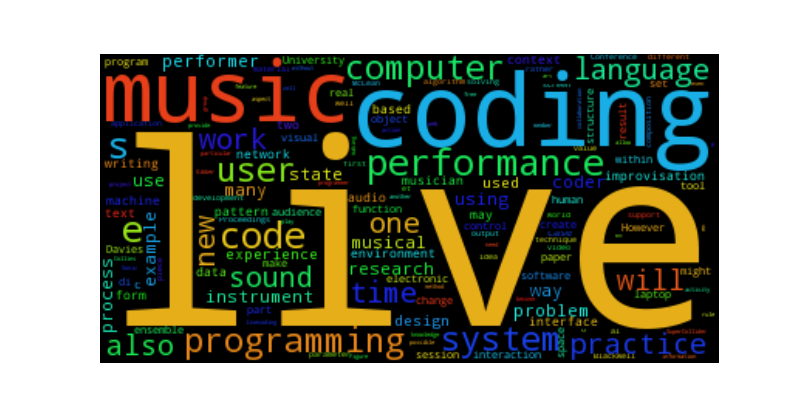
\includegraphics[scale=0.71]{./imagens/livecoding_cloud1.png}
\caption{Nuvem de palavras dos anais ICLC2015 \textbf{Fonte}: autor.}
\label{fig:nuvemlivecoding}
\end{center}
\end{figure}

\begin{table}
\caption{Tabela de classes qualitativas de termos utilizados nos anais do ICLC2015, agrupados por funções textuais.}
\small
    \begin{tabular}{ | p{1.5cm} | p{1.35cm} | p{2cm} | p{1.45cm} | p{1.45cm} | p{1.45cm} | p{1.45cm} | p{1.45cm} | p{1.25cm} |}
    \hline 
    \hline 

    \tiny \textbf{Número Qualitativo/Função} & \textbf{0} & \textbf{1}  & \textbf{2} & \textbf{3} & \textbf{4}  & \textbf{5} & \textbf{8} & \textbf{9}\\
    \hline 
    \hline 

    \tiny \textbf{Pessoas}  
    & - 
    & \tiny Collins, Blackwell, McLean, Grossi 
    & - 
    & - 
    & - 
    & -  
    & - 
    & - \\
    \hline

    \tiny \textbf{Aplicativos}
    & - 
    & \tiny SuperCollider, Gibber, SonicPi  
    & - 
    & - 
    & - 
    & -  
    & - 
    & \\
    \hline
    
    \tiny \textbf{Verbos}  
    & \tiny take, see, shared, networked, explore, made
    & \tiny make, provide, writing, solving, making
    & \tiny used
    & \tiny using, coding  
    & \tiny performer
    & - 
    & - 
    & -  \\
  \hline

     \tiny \textbf{Adjetivo ou numeral, ordinal}  
    & \tiny less, open, potential, similar, important, cognitive, virtual
    & \tiny first, real, electronic, visual, ensemble, possible, free, livecoding, aspect  
    & \tiny musical, many
    & \tiny new, one
    & - 
    & -  
    & \tiny live 
    & - \\
    \hline

    \tiny \textbf{Substantivo}  
    & \tiny Browser, point, approach, order, node, collaborative, number, source, present, community, server, framework, orchestra, digital, level, kind, type, memory, analysis, line, body, concept, technology, working, org, current, show, mean, end, processes, people, international
    & \tiny University, conference, proceedings, network, interface, environment, text, form, context, musician, space, paper, program, audience, function, change, control, human, laptop, interaction, structure, part, session, tool, result, create, object, case, algorithm, value, development, material, set, technique, parameter, idea, screen, video, application, support, composition, piece, knowledge, feature, cell, activity, art, action, information, method, web, rule, group, need, particular, project, allow, collaboration, programmer, member, play, output 
    & \tiny use, coder, process, state, example, way, software, research, problem, experience, design, improvisation, different, machine, pattern, audio
    & \tiny work, instrument
    & \tiny system, computer, user, language, time, practice, sound
    & \tiny programming
    & \tiny performance, code
    & \tiny ``live coding'', music  \\
    \hline
    \hline
   
    \end{tabular}
\label{tab:comparacao}
\end{table}

Uma breve análise da nuvem de palavras pode elucidar parte das questões-satélites. Na \autoref{tab:comparacao} filtrei parte dos resultados na nuvem de palavras por conjuntos de funções textuais -- sujeitos-humanos, sujeitos-ferramentas, verbos, adjetivos e substantivos -- e quantas vezes foram utilizados, em categorias qualitativas (0, menos usado e 9 o mais usado, sendo que 6 e 7 não apresentaram resultados). \footnote{O método de extração será explicado em um apêndice oportuno.}. 

No caso dos sujeitos-humanos, podemos ver nomes de Nick Collins e Alex McLean, praticantes responsáveis pela criação de um manifesto, em parceria com \citeonline{ward_live_2004}. Um fragmento deste manifesto será discutido no \autoref{cap:trabalhos_relacionados}. Pietro Grossi, é um personagem recentemente estudado por \citeonline{mori_pietro_2015} como um caso prematuro de \emph{live coding}, a partir do final da década de sessenta.

No caso dos sujeitos-ferramentas, destacamos o papel do \emph{SuperCollider}, já citado anteiormente, e do \emph{Gibber}\cite{roberts_gibber:_2012,wyse_viability_2014}\footnote{Disponível em \url{http://gibber.mat.ucsb.edu}}. Ambos são ambiente de programação para de síntese sonora e composição algorítmica. Um paradigma em comum destes ambientes: o procedimento de compilação de códigos conhecido como \emph{Just In Time} \cite{aycock_brief_2003}, que também será discutido no \autoref{cap:trabalhos_relacionados} como dispositivo técnico que permitiu a emancipação do \emph{livecoding}.

Os verbos fornecem informação sobre o comportamento dos improvisadores de códigos. Além da atividades como \emph{performatizar} e \emph{codificar}, é notável atividades sociais ligadas à visão, à escrita, à técnica, à lógica. Embora a Música seja a atividade proeminente do \emph{live coding}, não obtivemos resultados que retornassem, por exemplo, a palavra \emph{hearing}. Isso é significativo, e no \autoref{cap:trabalhos_relacionados}, exploro estas ações sob a ótica da Música de Processos de Steve Reich.

Já os adjetivos destacam características da prática, onde \emph{live} é a palavra-chave. Como será observado no \autoref{cap:trabalhos_relacionados}, a ação pode ocorrer em uma sala de concerto, um espaço público ou em uma casa noturna. Palavras como  \emph{electronic}, podem sugerir tanto uma música ``eletroacústica'', quanto gêneros de música para dançar. \emph{Visual} remete a uma característica tão fundamental quanto a Música. Um sem número de performances utilizam a projeção de telas de computadores como dispositivo de ``transparência''; isto é, uma ideologia de justificação do ato de improvisação. \emph{Ensemble} destaca uma a natureza de grupos. Poucas performances \emph{solo} são realizadas se comparadas às performances de \emph{duos}, \emph{trios}. 

Ainda no \autoref{cap:trabalhos_relacionados}, o \emph{live coding} se apropria da Música como Processo de Steve \citeonline{reich_music_1968} e da Música Generativa de Brian \citeonline{eno_music_1978} para justificar processos musicais com o virtuosismo de codificação\footnote{Neste trabalho criticamos esta visão. Ao que nos parece, ocorre uma confusão entre \emph{comportamentos criativos históricos} e, no caso do \emph{livecoding} emph{comportamentos criativos psicológicos}.}  

Palavras como \emph{university}, \emph{research} e \emph{technology}, e \emph{laptop} acusam não apenas uma prática artística, mas um Programa de Investigação Científica próprio. A esfera de pesquisa acadêmica permitiu ramos de desenvolvimento com linguagens de programação, cognição, inteligência artificial, semiologia, performance musical (improvisação), e mais recentemente, antropologia, conferindo à produção de \emph{live coding} espécie de autenticidade acadêmica.

\section{Sistemas Criativos, e o Universo de Conceitos}\label{sec:universo}

Uma sessão de \emph{live coding} é uma improvisação. Em seu artigo ``\emph{Music improvisation and creative systems}'', Alex \citeonline{mclean_music_2006},  articula a improvisação musical como uma atividade passível de formalização lógica. 

Este trabalho tem respaldo em outro, o artigo ``\emph{A preliminary framework for description, analysis and comparison of creative systems}'', de \citeonline{wiggins_framework_2006}. Por sua vez, define um mecanismo preliminar através do qual idéias de Margaret \citeonline{boden_creative_1990}, no livro ``The creative mind'' , são definidas formalmente.

\subsection{Sistemas Criativos}

O preceito para \emph{Universo de Conceitos} de McLean é a relação entre os \emph{Processos criativos} e \emph{Espaço conceitual} de Boden. Para Wiggins, ``Boden concebe o processo de criatividade como uma identificação e/ou localização de novos objetos conceituais em um espaço conceitual'' \cite[p.~450]{wiggins_framework_2006}\footnote{Tradução de \emph{Boden conceives the process of creativity as the identification and/or location of new conceptual objects in a conceptual space.}}.

Boden realiza duas taxonomias da criatividade. A primeira separa os comportamentos criativo em tipos H (históricos) e P (psicológicos). A segunda, separa o comportamento criativo em exploradores, e transformacionais. 

Comportamentos criativos do tipo H são aqueles tipos de conceitos historicamente novos, nunca inventados antes. Processos criativos do tipo P são os novos conceitos elaborados por uma pessoa\todo{\tiny Eu li uma parte do livro. Está no meu tablet, sem bateria e cabo para carregar. Assim que me organizar com isso, colocarei referências apropriadas.}. Por exemplo, os processos inventados em \emph{It's gonna rain} de Steve Reich, \emph{I'm sitting in a room} de Alvin Lucier ou as técnicas similares publicadas por Pauline \citeonline{oliveros_tape_1969} são comportamentos P-criativos que se tornaram H-criativos. Por outro lado consideramos, neste trabalho, os comportamentos criativos do \emph{livecoding} ainda como P-criativos. Carecem de tempo suficiente para serem considerados H-criativos.

Porém Wiggins poderia criticar ambas as visões (de Boden e a realizada no parágrafo anterior) da seguinte forma: ``pode ser possível, por exemplo, um comportamento ser P-criativo em uma sociedade, mas H-criativo em outra'' (\emph{Ibdem}, \emph{idem}). \footnote{Tradução de \emph{it would be possible, for example, for a creative behaviour to be only P-creative in one society, but H-creative in another.}}

A segunda taxonomia, que separa em comportamentos exploradores e transformacionais, lidam diretamente com o espaço conceitual. Se no primeiro caso este espaço é construído progressivamente com a elaboração de P-conceitos (o que pode ser observado em crianças), o transformacional é um comportamento que modifica o espaço conceitual existente, levando a filtrar quais são H-conceitos.

Para lidar formalmente com os Espaços Conceituais, Wiggins define ``criatividade'', ``computação criativa'', ``sistemas criativos'' e ``comportamentos criativos''. São apresentado na \autoref{tab:criatividade}

\begin{table}
\caption{Definições formais de criatividade por \citeonline[p.~451]{wiggins_framework_2006}}
\small
    \begin{tabular}{ | p{4cm} | p{11.25cm} |}
    \hline 
    \hline 

    \tiny{Criatividade} 
    & \tiny{``A performance de tarefas que, quando executados por um humano, são consideradas criativas''  \footnote{Tradução de \emph{The performance of tasks which, if performed by a human, would be deemed creative.}.}} \\
    \hline

    \tiny{Computação criativa} 
    & \tiny{``O estudo e suporte, através de meios e métodos computacionais, do comportamento exibido por sistemas naturais e artificiais, que são considerados criativos''. \footnote{Tradução de \emph{The study and support, through computational means and methods, of behaviour exhibited by natural and artificial systems, which would be deemed creative if exhibited by humans.}.}} \\
    \hline

    \tiny{Sistemas criativos} 
    & \tiny{``Uma coleção de processos, naturais ou automáticos, que são capazes de alcançarem ou simularem comportamentos que em humanos seria considerado criativo''} \\
    \hline

    \tiny{Comportamento Criativo} 
    & \tiny{``Um ou mais dos comportamentos exibidos por um sistema criativo''\footnote{Tradução de \emph{One or more of the behaviours exhibited by a creative system.}}} \\
    \hline
   
    \end{tabular}
\label{tab:criatividade}
\end{table}

Wiggins ainda define um \emph{Universo de possibilidades} no qual conceitos podem ser, em comportamentos transformacionais, contruídos para gerarem comportamentos H-criativos .

\subsection{Universo de conceitos ou de possibilidades}

\begin{citacao}
O universo, $\mathcal{U}$, é um espaço multidimensional, no qual dimensões são capazes de representar qualquer coisa, e todos os possíveis conceitos distintos correspondentes àqueles pontos em $\mathcal{U}$ (\ldots) Para tornar a proposta um espaço-tipo possível, permitirei que $\mathcal{U}$ contenha todos os conceitos abstratos, bem como os concretos, e que é possível representar os artefatos tanto completos e incompletos \cite[p.~451]{wiggins_framework_2006}.\footnote{Tradução de \emph{The universe, U, is a multidimensional space, whose dimensions are capable of representing anything, and all possible distinct concepts correspond with distinct points in U. (\ldots) To make the proposal as state-spacelike as possible, I allow that U contains all abstract concepts as well as all concrete ones, and that it is therefore possible to represent both complete and incomplete artefacts}}
\end{citacao}

Para diferenciar o Universo $\mathcal{U}$, do Espaço conceitual $\mathcal{C}$, Wiggins esclarece que Boden não reconhece de forma explícita $\mathcal{U}$, sendo que ``ela borra a distinção entre as regras que determinam a adesão do espaço (\ldots) e outras disposições que possam permitir a construção e/ou detecção de um conceito representado por um ponto no espaço'' \cite[p.~451]{wiggins_framework_2006}. Portanto, diferentes espaços conceituais estão contidos em $\mathcal{U}$;

Nas palavras de \citeonline{mclean_music_2006}, regras que validam a concepção do conceito no universo, são representadas como um conjunto$\mathcal{R}$. Regra que determinam estratégia de detecção (transversais) de um conceito no universo, são representados como o conjunto $\mathcal{T}$. Para lidar com estas regras, é necessária uma \emph{linguagem} $\mathcal{L}$ para expressá-las. Nas palavras de Wiggins: ``um conjunto de sequências compostas por algum alfabeto $\mathcal{A}$''\footnote{Tradução de \emph{it as the set of all sequences composed of some alphabet, A.}}

A \autoref{tab:universodeconceitos} ilustra os termos até agora trabalhados por McLean:

\begin{table}[!h]
\caption{Definições formais do Universo de possibilidades de \citeonline{wiggins_framework_2006}, ou Universo de Conceitos por \citeonline{mclean_music_2006}.}
\small
    \begin{tabular}{ | p{4cm} | p{5.5cm} | p{5.5cm} |}
    \hline 
    \hline 

    \tiny{Representação} 
    & \tiny{Nome}      
    & \tiny{Significado} \\
    \hline

    $c$
    & \tiny{Conceito} 
    & \tiny{Uma instância de um conceito, abstrato ou concreto \cite{wiggins_framework_2006}.} \\
    \hline

    $\mathcal{U}$
    & \tiny{Universo de Conceitos} 
    & \tiny{Superconjunto não restrito de conceitos. \cite{wiggins_framework_2006}. ``Um universo de todos conceitos possíveis'' \cite{mclean_music_2006} \footnote{Tradução de \emph{A universe of all possible concepts}.}}\\
    \hline

    $\mathcal{L}$
    & \tiny{Linguagem} 
    & \tiny{Linguagem utilizada para expressar regras.} \\
    \hline

    $\mathcal{A}$
    & \tiny{Alfabeto} 
    & \tiny{Alfabeto da linguagen que contêm caracteres apropriados} \\
    \hline

    $\mathcal{R}$
    & \tiny{Regras de validação} 
    & \tiny{Validam os conceitos em um universo, se apropriados ou não para o espaço trabalhado.} \\
    \hline

    $[[.]]$
    & \tiny{Função de interpretação} 
    & \tiny{``Uma função parcial de $\mathcal{L}$ para funções que resultam em números reais entre [0, 1] (\ldots) 0.5 $[$ou maior$]$ significa uma verdade booleana e menos que 0.5 siginifica uma falsidade booleana; a necessidade disso para valores reais se tornará clara abaixo'' \cite[p.~452]{wiggins_framework_2006}\footnote{Tradução de \emph{(\ldots) a partial function from $\mathcal{L}$ to functions yielding real numbers in [0, 1]. (\ldots) 0.5 to mean Boolean true and less than 0.5 to mean Boolean false; the need for the real values will become clear below}.}}\\
    \hline

     $[[\mathcal{R}]]$
    & \tiny{Regras de validação} 
    & \tiny{``Uma função que interpreta $\mathcal{R}$, resultando em uma função indicando aderência ao conceito em $\mathcal{R}$''\footnote{Tradução de \emph{A function interpreting $\mathcal{R}$, resulting in a function indicating adherence of a concept to $\mathcal{R}$}}} \\
    \hline

     $\mathcal{C} = [[\mathcal{R}]](\mathcal{U}) $
    & \tiny{Espaço Conceitual} 
    & \tiny{``Todos espaços conceituais são um subconjunto não-estrito de $\mathcal{U}$''\footnote{Tradução de \emph{All conceptual spaces are non-strict subset}.}. Um subconjunto contido em $\mathcal{U}$ \cite{wiggins_framework_2006}. Uma função que interpreta $\mathcal{R}$, resultando em uma função que indica aderência ao conceito em $\mathcal{R}$ \footnote{Tradução de \emph{A function interpreting $\mathcal{R}$, resulting in a function indicating adherence of a concept to $\mathcal{R}$}.} } \\
    \hline

    $\mathcal{T}$
    & \tiny{Regras de detecção} 
    & \tiny{``Regras definidas dentro de $\mathcal{L}$ para definir estratégias transversais para localizar conceitos dentro de $\mathcal{U}$'' \cite{mclean_music_2006}\footnote{Tradução de \emph{Rules defined within $\mathcal{L}$ to define a traversal strategy to locate concepts within $\mathcal{U}$ }}} \\
    \hline

    $\mathcal{E}$
    & \tiny{Regras de qualidade} 
    & \tiny{``(\ldots) conjunto de regras que permitem-nos avaliar qualquer conceito que nós encontramos em $\mathcal{C}$ e determinar sua qualidade, de acordo com critérios que nós considerarmos apropriados'' \cite[p.453]{wiggins_framework_2006}\footnote{Tradução de \emph{(\ldots) set of rules which allows us to evaluate any concept we find in C and determine its quality, according to whatever criteria we may consider appropriate.}}``Regras definidas dentro de $\mathcal{L}$ para avaliar a qualidade ou a desejabilidade do conceito $c$'' \cite{mclean_music_2006}\footnote{Tradução de \emph{Rules defined within $\mathcal{L}$ which evaluate the quality or desirability of a concept $c$.}}}\\
    \hline

    $<<<\mathcal{R}, \mathcal{T}, \mathcal{E}>>>$
    & \tiny{Função de interpretação} 
    & \tiny{Uma regra necessária para definir o espaço conceitual, ``independentemente da ordem, mas também, ficcionalmente, enumerá-los em uma ordem particular, sob o controle de $\mathcal{T}$ -- isto é cricial para a simulação de um comportamento criativo de um $\mathcal{T}$ particular \cite{wiggins_framework_2006} \footnote{Tradução de \emph{We need a means not just of defining the conceptual space, irrespective of order, but also, at least notionally, of enumerating it, in a particular order, under the control of $\mathcal{T}$ -- this is crucial to the simulation of a particular creative behaviour by a particular $\mathcal{T}$.}}. ``Uma função que interpreta a estratégia transversal $\mathcal{T}$, informada por $\mathcal{R}$ e $\mathcal{E}$ . Opera sobre um subconjunto ordenado de $mathcal{U}$ (do qual tem acesso randômico) e resulta em outro subconjunto ordenado de $\mathcal{U}$.''\footnote{Tradução de \emph{A function interpreting the traversal strategy $\mathcal{T}$, informed by $\mathcal{R}$ and $\mathcal{E}$ . It operates upon anordered subset of $mathcal{U}$ (of which it has random access) and results in another ordered subset of $\mathcal{U}$.}}} \\
    \hline
    \hline
   
    \end{tabular}
\label{tab:universodeconceitos}
\end{table}



\section{O modelo de improvisação}

TODO ...

\section{Exemplo concreto da multiplicadade em um universo de possibilidades}

Durante a pesquisa, investigamos um campo específico, mas que não será utilizado como trabalho final. Por outro lado, permitiu visualizar os conceitos  $c$ de universo de conceitos $U$ em uma mídia social (\emph{Soundcloud}).

As \autoref{fig:pacotao}, \autoref{fig:pacotao2}, ilustram a multiplicidade de conceitos $c$. Agrupados por data, país, cidade e \emph{hashtags} que ``delimitam'' um gênero musical, possibilitaram reduzir um pouco o estudo, mas não completamente.

\begin{figure}[h]
\begin{center}
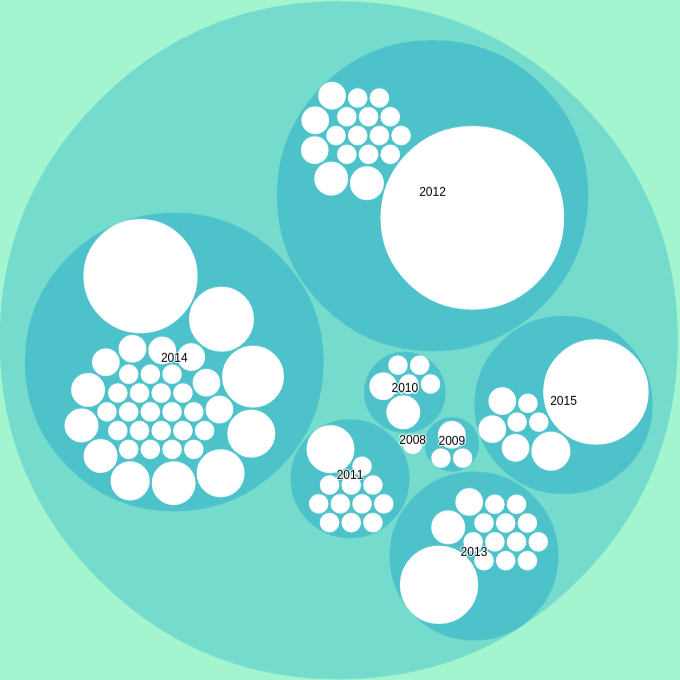
\includegraphics[scale=0.6]{./imagens/zoomable_circle_packing_genre_year_livecoding.png}
\caption{Empacotamento de informações a respeito de gênero musical a partir de anos de produção}
\label{fig:pacotao}
\end{center}
\end{figure}

Os seguintes os termos delimitados foram: \begin{inparaenum}[\itshape a)\upshape]
\item \emph{livecoding}/\emph{live-coding}: dados coerentes com a bibliografia pesquisada\footnote{A exclusão do termo \emph{live code/live coding} foi feita pois a separação criava uma ambiguidade de busca no \emph{Soundcloud}, isto é, \emph{live} poderia não se referir ao que pesquisamos por \emph{livecoding}.};
\item \emph{algorave}/\emph{algopop}: parte considerável da produção do \emph{livecoding} realizada em ambientes noturnos, informais ou de entretenimento (possue relação com o elemento dança);
\item \emph{bytebeat}: parte considerável de uma técnica de programação musical descrita pela primeira vez por \citeonline{heikkila_discovering_2011} e aplicada no \emph{livecoding}, isto é, apenas um fragmento dessa prodção pode se encaixar como \emph{livecoding} (um desses programas é o \emph{Wavepot});
\item \emph{algorithmic music}:música algorítmica, seguindo a subdivisão Música Gerada por Computador, ou \emph{Computer Generated Music}\cite{cope_prefacio_2008}.
\end{inparaenum}

\begin{figure}[h]
\begin{center}
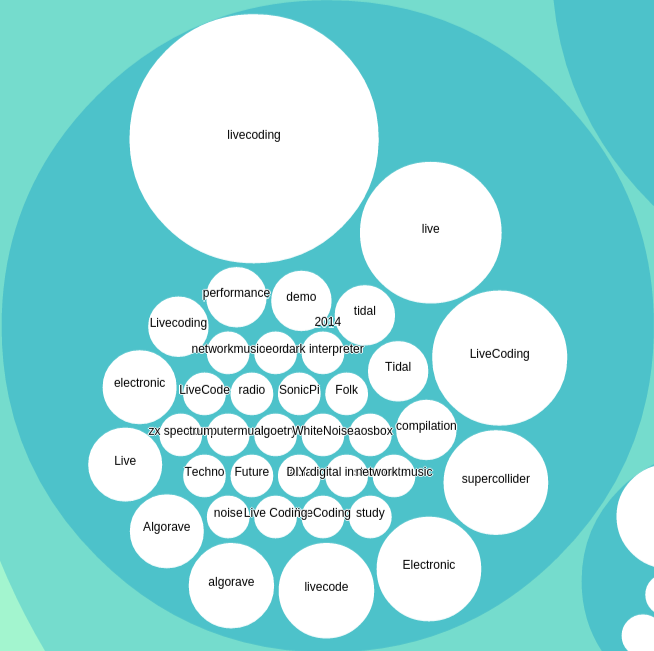
\includegraphics[scale=0.6]{./imagens/zoomable_circle_packing_genre_year_livecoding2.png}
\caption{Detalhamento de informações a respeito de gênero musical a partir de anos de produção}
\label{fig:pacotao2}
\end{center}
\end{figure}

Os dados levantados são de janeiro e fevereiro de 2015; não realizamos mais levantamentos. Os motivos foram: \begin{inparaenum}[\itshape i)\upshape]
\item a dificuldade de análise das assimetrias observadas, que requerem maior experiência com técnicas estatísticas.
\item os dados ilustram as variedades de categorizações musicais no \emph{live coding}. Pode ser interessante observar se tais variedades se aplicam em um único \emph{live coder}.
\end{inparaenum}

\begin{figure}
\begin{center}
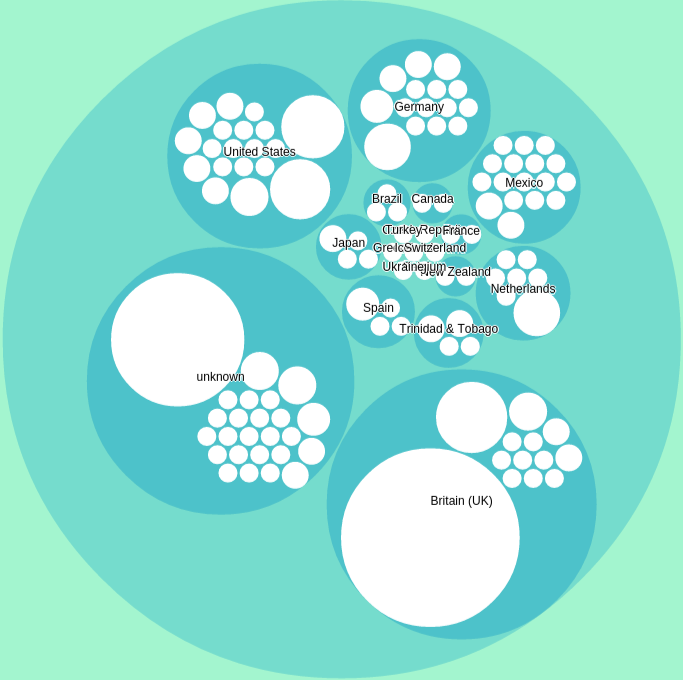
\includegraphics[scale=0.6]{./imagens/zoomable_circle_packing_genre_year_livecoding3.png}
\caption{Empacotamento de informações a respeito de gênero musical a partir de países onde ocorreram as produções}
\label{fig:pacotao3}
\end{center}
\end{figure}

Antes de discutir três casos específicos de um \emph{live coder} (Sorensen), contextualizamos os \emph{live coding} no \autoref{cap:trabalhos_relacionados}. Alguns precedentes históricos do \emph{live coding}, como \emph{GROOVE}, o compositor \emph{Pietro Grossi}, a \emph{Live Computer Music} da Baía de São Franscisco entre os anos 70 e 80 nos Estados Unidos, e a emancipação de uma organização, TOPLAP\footnote{Disponível em \url{http://www.toplap.org}.}, e o destaque de \emph{live coders} ingleses, foram fatores para descrever, neste trabalho, o \emph{live coding} como técnica de improvisação artística original de um Norte político e econômico; delimitar o \emph{live coding} como um Programa de Investigação Científica em universidades; ou descrever o \emph{live coding} como dispositivo de improvisação para replicação de categorizações musicais.

\begin{figure}
\begin{center}
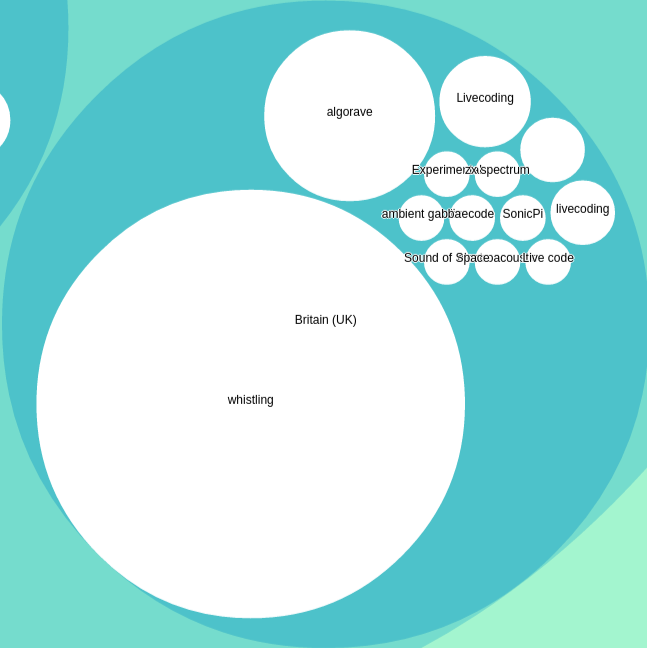
\includegraphics[scale=0.6]{./imagens/zoomable_circle_packing_genre_year_livecoding4.png}
\caption{Detalhamento de informações a respeito de gênero musical a partir de países onde ocorreram as produções.}
\label{fig:pacotao4}
\end{center}
\end{figure}